\subsection{Results}
\label{sec:results}

\newcommand{\takeaway}[1]{
\vspace{6pt}
\noindent\fbox{\parbox{0.98\columnwidth}{#1}}
\vspace{6pt}
}

\begin{figure*}
  \centering
  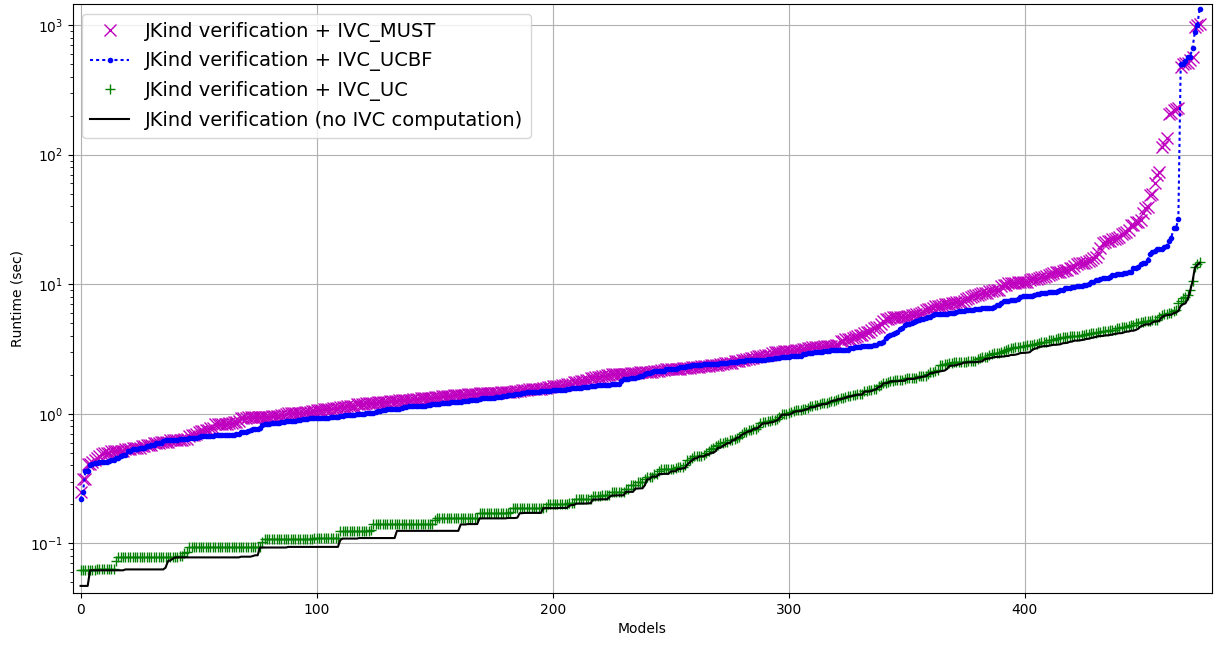
\includegraphics[width=0.85\textwidth]{figs/timing_analyses_all_sorted.png}
  \vspace{-0.1in}
  \caption{Runtime of different analyses}\label{fig:runtimeall}
\end{figure*}

\begin{figure*}
  \centering
  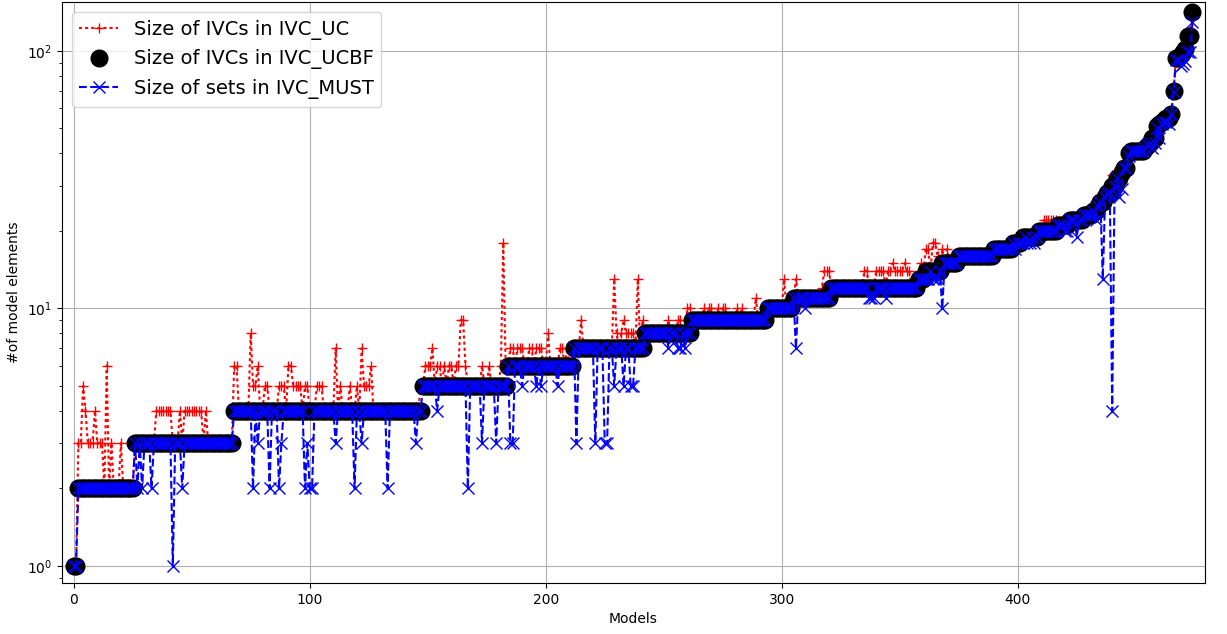
\includegraphics[width=0.85\textwidth]{figs/size.png}
  \vspace{-0.1in}
  \caption{Runtime of different analyses}\label{fig:size}
\end{figure*}

In this section, we examine our experimental results to address the aforementioned research questions.

\textbf{RQ1}). First we examine the performance overhead of the \ucalg algorithm over the time necessary to find a proof using inductive model checking. To measure the performance overhead of an algorithm, we executed it over the proof generated by the {\em fastest} JKind option. Tables~\ref{tab:runtime-ucalg}
and~\ref{tab:overhead-ucalg} represent both the
computation time for coverage analysis
and the overhead imposed by the algorithms.

\begin{table}
  \caption{runtime of different coverage analyses}
  \centering
  \begin{tabular}{ |c||c|c|c|c| }
    \hline
     runtime (sec) & min & max & mean & stdev \\[0.5ex]
    \hline\hline
    %proof time   & 0.047 & 14.617 & 1.299 & 1.940 \\[0.5ex]
    \ucalg &   0.0  & 1.422  & 0.084 & 0.184 \\[0.5ex]
    \mustalg & 0.14 & 997.386 &  19.342 & 97.818 \\[0.5ex]
    \ucbfalg& 0.248 & 1323.515 &  17.247 & 104.838 \\[0.5ex]
    \hline
  \end{tabular} \\
  \label{tab:runtime-ucalg}
\end{table}

\begin{table}
  \caption{Overhead of different coverage analyses}
  \centering
  \begin{tabular}{ |c||c|c|c|c| }
    \hline
     Algorithm & min & max & mean & stdev \\[0.5ex]
    \hline
    \ucalg &   0.0\%  & 100\%  & 10.226\% & 11.718\% \\[0.5ex]
    \mustalg & 13.732\% & 10530.769\% &  1081.099\% & 1613.264\% \\[0.5ex]
    \ucbfalg& 14.092\% & 11124.432\% &  882.018\% & 1512.071\% \\[0.5ex]
    \hline
  \end{tabular}
  \label{tab:overhead-ucalg}
\end{table}

Fig.~\ref{fig:runtimeall} allows a visualization of the runtime of different coverage analyses
in comparison with the proof time, which indicates the overhead induced by each algorithm.

\takeaway{Coverage analysis using \ucalg is quite efficient with a low overhead compared to \mustalg .}


\textbf{RQ2}). When a coverage metric brings about lower coverage scores on average,
it is said that metric is harder to satisfy. In the Second research question,
we are interested in comparing this aspect of the proposed metrics. To address \textbf{RQ2}, we evaluate the experimental results from different perspectives. The first thing we calculated is the size of the output sets generated by each algorithm: in average, size of the output sets generated by \ucalg are 1.104 times bigger than the minimal sets obtained from \ucbfalg, while the output sets of \mustalg are averagely 0.958 smaller than the \ucbfalg, which shows \mustalg is harder to satisfy, and also does not maintain provability. Fig. \ref{fig:size} is a visualization of the size of the set of covered elements by different algorithms. The graph shows the degree of under-approximation by \mustalg as well as the degree of over-approximation by \ucalg. Note that \ucbfalg is accurate. It means that \ucalg might report some elements as covered, while they are not. And, \mustalg reports some elements uncovered, while they are.

Next, we provide a report on the coverage score of the analyses in Table~\ref{tab:cov-score}. In addition, to investigate
the relationship between provability and different coverage notions,
we were interested in the number of models in the benchmark for which $\mustalg (\Gamma \vdash R) \nvdash R$.
Obviously the specifications are provable by 100\% of the support sets computed by \ucalg (and \ucbfalg).
As for the \mustalg algorithm, the specifications were not provable by the \emph{must} set (i.e. the output of \mustalg) of 18\% of the models in the benchmarks.

\begin{table}
  \caption{Overhead of different coverage analyses}
  \centering
  \begin{tabular}{ |c||c|c|c|c| }
    \hline
     score & min & max & mean & stdev \\[0.5ex]
    \hline\hline
    \ucalg &   0.002  & 1.0  &  0.466 & 0.302 \\[0.5ex]
    \mustalg & 0.002 & 1.0 &  0.414 & 0.290 \\[0.5ex]
    \ucbfalg& 0.002 & 1.0 &  0.429 & 0.288 \\[0.5ex]
    \hline
  \end{tabular}
  \label{tab:cov-score}
\end{table}

\takeaway{On average, coverage analysis using \ucalg is 115\% easier to satisfy,
compared to \mustalg. In the assessment of completeness, \ucalg has an average error rate of $+8\%$,
while the average error rate of \mustalg is $-3\%$.}

\takeaway{\mustalg failed to maintain provability on 20\% of the benchmarks.} 